% TU Delft Beamer template
% Author: Maarten Abbink
% Delft University of Technology
% March 2014
% Version 2.0
% Based on original version 1.0 of Carl Schneider
\documentclass{beamer}
\usepackage[english]{babel}
\usepackage{calc}
\usepackage[absolute,overlay]{textpos}
\usepackage{amsmath}
\usepackage{tikz}
\usepackage{qtree}
\usepackage{soul}
\usepackage{threeparttable}
\usepackage{algorithm2e}
\usepackage{minibox}
\usepackage[gen]{eurosym}
\mode<presentation>{\usetheme{tud}}

\SetKwProg{Fn}{Function}{ :}{end}
\SetKw{Break}{break}

\title[]{Reengineering Alitheia Core}
\institute[TU Delft]{Software Reengineering - IN4189}
\author{Anton Bouter - Martijn den Hoedt}
\date{\today}

% Insert frame before each subsection (requires 2 latex runs)
\AtBeginSubsection[] {
	\begin{frame}<beamer>\frametitle{\titleSubsec}
		\tableofcontents[currentsection,currentsubsection]  % Generation of the Table of Contents
	\end{frame}
}
% Define the title of each inserted pre-subsection frame
\newcommand*\titleSubsec{Next Subsection}
% Define the title of the "Table of Contents" frame
\newcommand*\titleTOC{Outline}

% define a symbol which can be removed if you don't need it
\newcommand{\field}[1]{\mathbb{#1}}
\newcommand{\Zset}{\field{Z}}

\begin{document}

% remove the next line if you don't want a background image
\setbeamertemplate{footline}{\usebeamertemplate*{minimal footline}}
\frame{\titlepage}

\setbeamertemplate{footline}{\usebeamertemplate*{minimal footline}}
\begin{frame}
    \frametitle{Outline}
    \begin{itemize}
        \item Shortcomings
        \item Improvements
        \item Recommendations
        \item Conclusions
    \end{itemize}
\end{frame}

\begin{frame}
    \frametitle{Scenario}
    \begin{columns}
    
        \begin{column}{0.3\textwidth}
        		\centering
            
\includegraphics[width=0.5\textwidth]{../img/personIcon.png}
            \\ \vspace{30px}
            \centering
            \includegraphics<1>[width=0.5\textwidth]{../img/personIcon.png}
            \tikz\node[opacity=0.3]{\includegraphics<2->[width=0.5\textwidth]{../img/personIcon.png}};
        \end{column}
        
        \begin{column}{0.3\textwidth}
        		\centering
            
\includegraphics[width=\textwidth]{../img/sqo-oss.png}
        \end{column}
        
        \begin{column}{0.3\textwidth}
        		\centering
            \includegraphics<-4>[width=0.5\textwidth]{../img/personIcon.png}
            \tikz\node[opacity=0.3]{\includegraphics<5->[width=0.5\textwidth]{../img/personIcon.png}};
            \\ \vspace{30px}
            \includegraphics<-2>[width=0.5\textwidth]{../img/personIcon.png}
            \tikz\node[opacity=0.3]{\includegraphics<3>[width=0.5\textwidth]{../img/personIcon.png}};
            \includegraphics<4->[width=0.5\textwidth]{../img/personIcon2.png}
        \end{column}
        
    \end{columns}
\end{frame}

\begin{frame}
    \frametitle{Shortcomings - Single Responsibility Principle}
    \begin{itemize}
        \item Every software entity should have a single purpose.
        \item inCode tool
    \end{itemize}
    
    \begin{figure}
    	\centering
    	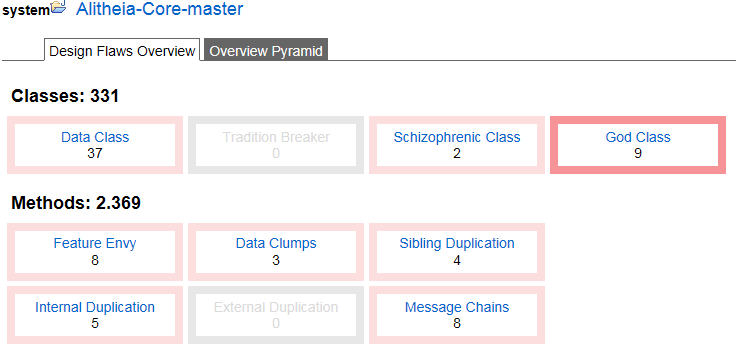
\includegraphics[width=0.8\textwidth]{../img/inCodeOverview.png}
    \end{figure}
\end{frame}

\begin{frame}
    \frametitle{Improvements - Single Responsibility Principle}
    \begin{itemize}
        \item Split GitUpdater into 4 classes.
    \end{itemize}
    
    \begin{figure}
    	\centering
    	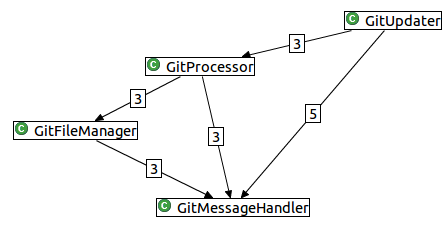
\includegraphics[width=0.8\textwidth]{../img/gitUpdaterDependencies.png}
    \end{figure}
\end{frame}

\begin{frame}
    \frametitle{Shortcomings - Dependency Inversion \\ Principle}
	\begin{columns}
	
	\begin{column}{0.4\textwidth}    
    		\begin{itemize}
    		    \item High-level modules should not depend on low-level modules.
    		    \item STAN Eclipse plugin
    		\end{itemize}
    \end{column}
    
    \begin{column}{0.6\textwidth}
    		\begin{figure}
    		\centering
    		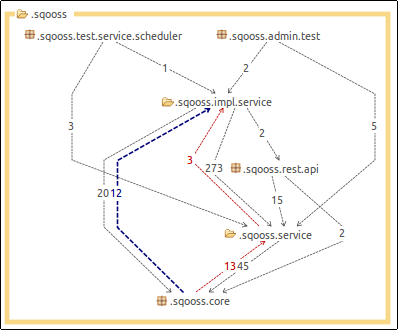
\includegraphics[width=\textwidth]{../img/impl-depedency.png}
    		\end{figure}
    \end{column}
    
    \end{columns}
\end{frame}

\begin{frame}
    \frametitle{Shortcomings - Acyclic Dependency Principle}
    \begin{itemize}
        \item If A depends on B, B should not depend on A.
        \item STAN Eclipse plugin
    \end{itemize}
    
    \begin{figure}
    	\centering
    	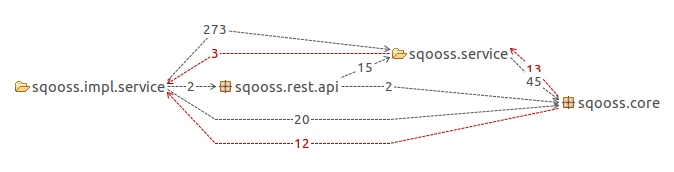
\includegraphics[width=\textwidth]{../img/cycle1.png}
    \end{figure}
\end{frame}

\begin{frame}
    \frametitle{Improvements - Acyclic Dependency Principle}
    Solved cyclic dependencies:
    \begin{itemize}
        \item service.abstractmetric
        \item service.fds
    \end{itemize}
    
    \begin{figure}
    	\centering
        \includegraphics<1>[width=0.8\textwidth]{../img/fds-before.png}
    	\includegraphics<2>[width=\textwidth]{../img/fds-after.png}
    \end{figure}
\end{frame}

\begin{frame}
    \frametitle{Shortcomings - Lack of tests}
    \begin{itemize}
        \item EclEmma tool
        \item \textbf{Terrible coverage of 1.7\%!}
        
    \end{itemize}
    \begin{figure}
    	\centering
    		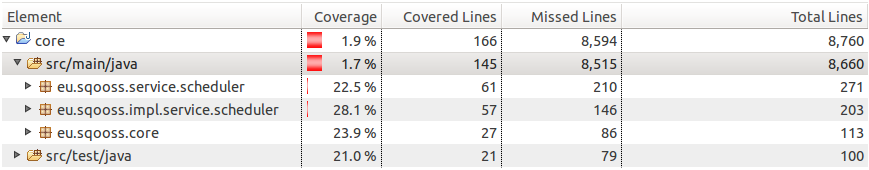
\includegraphics[width=\textwidth]{../img/coreCoverageBefore.png}
    \end{figure}
\end{frame}

\begin{frame}
    \frametitle{Improvements - Tests}
    \begin{itemize}
        \item Core coverage of 11.0\%.
    \end{itemize}
    
    \begin{figure}
    	\centering
    		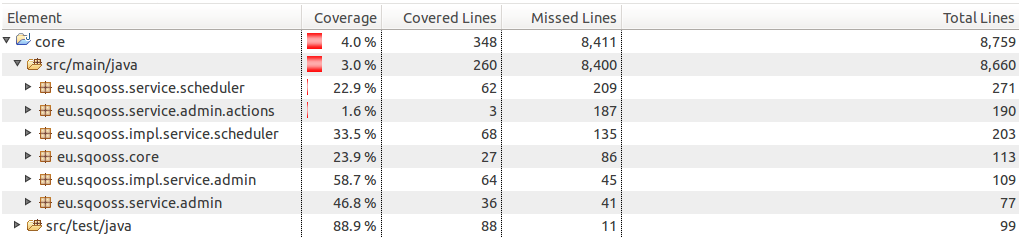
\includegraphics[width=\textwidth]{../img/coreCoverageAfter.png}
    \end{figure}
\end{frame}

\begin{frame}
    \frametitle{Recommendations}
    \begin{itemize}
    		\item Create tests.
    		\item<2-> Create more tests.
    		\item<3-> Perform more refactorings to fix e.g. SRP and DIP problems.
    		\item<4-> $\euro{}$ 15.000 to hire additional developers.
    \end{itemize}
\end{frame}

\begin{frame}
    \frametitle{Conclusion}
    \begin{itemize}
    		\item Many problems that affect maintainability.
    		\item Some improvements have been made.
    		\item $\euro{}$ 15.000 required to keep the system maintainable.
    \end{itemize}
\end{frame}

\begin{frame}
    \frametitle{Questions}
    \hspace{.25\linewidth}
    \Huge{Questions?}
\end{frame}

\end{document}
